\documentclass{standalone}
\usepackage{tikz}
\usetikzlibrary{arrows.meta,babel,positioning}
\tikzset{%
    >={Latex[width=2mm,length=2mm]},
    base/.style = {
        rectangle, rounded corners, draw=black, minimum width=4cm,
        minimum height=1cm, text centered, font=\sffamily
    },
    startLoop/.style = {base, fill=blue!30},
    repeat/.style = {base, fill=green!30},
    process/.style = {base, minimum width=2.5cm, fill=orange!15, font=\ttfamily},
}
\begin{document}
    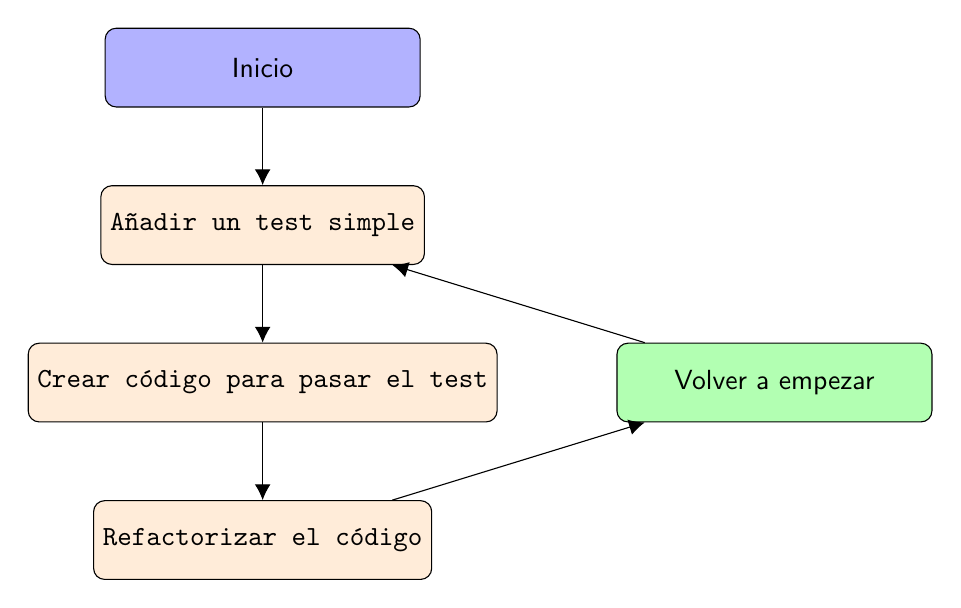
\begin{tikzpicture}[
        node distance=1.5cm,
        every node/.style={fill=white, font=\sffamily},
        align=center
    ]
        % Nodes position
        \node (start)         [startLoop]
                                {Inicio};
        \node (addTest)       [process, below of=start, yshift=-0.5cm]
                                {Añadir un test simple};
        \node (addSimpleCode) [process, below of=addTest, yshift=-0.5cm]
                                {Crear código para pasar el test};
        \node (refactorCode)  [process, below of=addSimpleCode, yshift=-0.5cm]
                                {Refactorizar el código};
        \node (repeat)        [repeat, right of=addSimpleCode, xshift=5cm]
                                {Volver a empezar};

        % Arrow specification
        \draw[->]         (start) -- (addTest);
        \draw[->]       (addTest) -- (addSimpleCode);
        \draw[->] (addSimpleCode) -- (refactorCode);
        \draw[->]  (refactorCode) -- (repeat);
        \draw[->]        (repeat) -- (addTest);
    \end{tikzpicture}
\end{document}